\subsection{Zjednodušený model systému}
Nyní vytvoříme zjednodušený 1 DoF model reálného systému (viz obrázek č. \ref{fig:1 DoF schéma robota}), který poslouží pro názornější vizualizaci výsledků dosažených navrženými algoritmy a~jejich snazší otestování a~také porovnání různých přístupů.
Uvažujeme rameno o~délce $l$ a~hmotnosti $m$, které je na jednom konci
ukotvené na hřídeli prostřednictvím rotačního kloubu s~pohonem generující moment síly (točivý moment) $T$. Abychom mohli
nějakým způsobem lépe simulovat změnu fyzikálních parametrů, zavedeme do modelu
také pružnost $k$ a~koeficient tlumení $b$ pohybu ramene. Výsledné schéma je na
obrázku č. \ref{fig:1 DoF schéma robota}.

\begin{figure}[H]
    \centering
    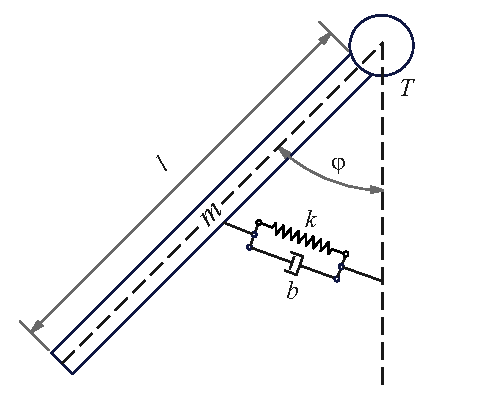
\includegraphics{Img/Drawing.pdf}
    \caption{Schéma zjednodušeného ramene robota}
    \label{fig:1 DoF schéma robota}
\end{figure}
Budeme vycházet z~Newtonovo druhého pohybového zákona pro rotační pohyb --- konkrétně z~rovnice pro moment síly $\bm{M}$, rovnice pro moment hybnosti $\bm{L}$
a jejich vzájemného vztahu:
\begin{align}
    \bm{M} & = \bm{r}\times\bm{F}                             \\
    \bm{L} & = \bm{r}\times\bm{p} = \bm{r}\times m\cdot\bm{v} \\
    \bm{M} & = \frac{d\bm{L}}{dt}
\end{align}
Dosazením parametrů našeho modelu dostáváme:
\begin{align}
    M & = -mgl\cdot\sin(\varphi(t)) -k\cdot\varphi(t) - b \cdot\dot{\varphi}(t) + T(t) \\
    L & =  ml^2\cdot\dot\varphi(t)
\end{align}
Výsledný model je popsán diferenciální rovnicí:
\begin{align}
    \dot{L}                    & =  M                                                                                        \\
    ml^2\cdot\ddot\varphi(t)   & = -mgl\cdot\sin(\varphi(t)) -k\cdot\varphi(t) - b \cdot\dot{\varphi}(t) + T(t)              \\
    \implies \ddot{\varphi}(t) & =  \frac{- mgl\cdot\sin(\varphi(t)) - k\cdot\varphi(t) -b\cdot\dot\varphi(t) + T(t)}{l^2m }
\end{align}
Na tomto modelu můžeme například vykreslit potřebný točivý moment $T$ v~ustáleném stavu ($\ddot{\varphi} = \dot{\varphi} = 0$) pro daný konstantní úhel $\varphi$ na základě různých fyzikálních para\-metrů --- viz obrázek č.~\ref{fig:1 DoF pro různé parametry}. Tímto můžeme simulovat změny fyzických parametrů, které časem probíhají i~na reálném stroji a~také na výsledcích můžeme později odzkoušet interpolační/aproximační algoritmy. V~zásadě se jedná o~proudovou kalibrační tabulku pro náš 1 DoF model, protože točivý moment $T$ je přímo úměrný proudu.
\begin{figure}[H]
    \centering
    \includegraphics{Generated/1 DoF model - změny parametrů.pdf}
    \caption{Potřebný točivý moment motoru pro dosažení úhlu $\varphi$ pro různé parametry 1 DoF modelu}
    \label{fig:1 DoF pro různé parametry}
\end{figure}